\documentclass[12pt]{article}
\usepackage[margin=1in]{geometry}
\usepackage{amsmath}
\usepackage{tikz}

\setlength{\parindent}{0pt}
\setlength{\parskip}{8pt}

\title{Unit 10: Quadratic Graphs \& Completing the Square}
\author{
	Student: SA\\
	Tutor: Rachel Eglash}
\date{November 15, 2025}

\begin{document}
	
	\maketitle
    
    \newpage

	\section*{Session 10.1: \\ Quadratic Graphs (Vertex, Axis, Intercepts)}

	\section*{Quick Reference: Quadratic Functions}

		\subsection*{Standard Form of a Quadratic}

			$y = ax^2 + bx + c$  where $a$, $b$, and $c$ are constants and $a \neq 0$

		\subsection*{Key Features of a Parabola}

			\textbf{Vertex:} The highest or lowest point on the parabola\\

			\textbf{Axis of Symmetry:} The vertical line through the vertex
            
            Formula: $x = -\frac{b}{2a}$\\

			\textbf{Direction:}
            
            If $a > 0$, parabola opens upward (vertex is minimum)

            If $a < 0$, parabola opens downward (vertex is maximum)\\

			\textbf{$y$-intercept:} Where the graph crosses the $y$-axis
            
            Set $x = 0$, solve for $y$. Point: $(0, c)$\\

			\textbf{$x$-intercepts:} Where the graph crosses the $x$-axis
            
            Set $y = 0$, solve for $x$ (factor or use other methods)

		\subsection*{Finding the Vertex from Standard Form}

			Given $y = ax^2 + bx + c$:

			\textbf{Step 1:} Find $x$-coordinate of vertex: $x = -\frac{b}{2a}$

			\textbf{Step 2:} Substitute this $x$-value into the equation to find $y$

			\textbf{Step 3:} Vertex is at point $\left(-\frac{b}{2a}, y\right)$

			\newpage

	\section*{Homework 10.1: \\ Quadratic Graphs — Vertex, Axis, Intercepts}

		\subsection*{Part A: Identify Key Features}

			For each quadratic function, identify:
			\begin{itemize}
				\item Direction (opens up or down)
				\item $y$-intercept
				\item Axis of symmetry
				\item Vertex
			\end{itemize}

			Show your work for finding the vertex.\\\\

			\textbf{Problem 1:}
            
            $y = x^2 + 6x + 5$

			\vspace{1cm}

			Direction: \underline{\hspace{2in}}

			$y$-intercept: \underline{\hspace{2in}}

			Axis of symmetry: \underline{\hspace{2in}}

			Work for vertex:

			\vspace{3cm}

			Vertex: \underline{\hspace{2in}}

			\newpage

			\textbf{Problem 2:}
            
            $y = -x^2 + 4x - 3$

			\vspace{1cm}

			Direction: \underline{\hspace{2in}}

			$y$-intercept: \underline{\hspace{2in}}

			Axis of symmetry: \underline{\hspace{2in}}

			Work for vertex:

			\vspace{3cm}

			Vertex: \underline{\hspace{2in}}

			\vspace{2cm}

			\textbf{Problem 3:}
            
            $y = 2x^2 - 8x + 3$

			\vspace{1cm}

			Direction: \underline{\hspace{2in}}

			$y$-intercept: \underline{\hspace{2in}}

			Axis of symmetry: \underline{\hspace{2in}}

			Work for vertex:

			\vspace{3cm}

			Vertex: \underline{\hspace{2in}}

			\newpage

		\subsection*{Part B: Find $x$-intercepts}

			Find the $x$-intercepts by setting $y = 0$ and factoring.\\\\

			\textbf{Problem 4:}
            
            $y = x^2 + 6x + 5$

			\vspace{4cm}

			$x$-intercepts: \underline{\hspace{3in}}

			\vspace{1cm}

			\textbf{Problem 5:}
            
            $y = x^2 - 9$

			\vspace{4cm}

			$x$-intercepts: \underline{\hspace{3in}}

			\newpage

			\textbf{Problem 6:}
            
            $y = x^2 + 5x + 6$

			\vspace{4cm}

			$x$-intercepts: \underline{\hspace{3in}}

			\vspace{1cm}

			\textbf{Problem 7:}
            
            $y = -x^2 + 2x + 8$

			\vspace{4cm}

			$x$-intercepts: \underline{\hspace{3in}}

			\newpage

		\subsection*{Part C: Graph from Key Features}

			Use the key features you found to sketch a graph.\\

			For each function:
			\begin{itemize}
				\item Plot the vertex
				\item Draw the axis of symmetry
				\item Plot the $y$-intercept
				\item Plot the $x$-intercepts (if you found them)
				\item Sketch the parabola
			\end{itemize}

			\textbf{Problem 8:}
            
            Graph $y = x^2 + 6x + 5$ using your work from Problems 1 and 4.

			\vspace{0.5cm}

			\begin{center}
			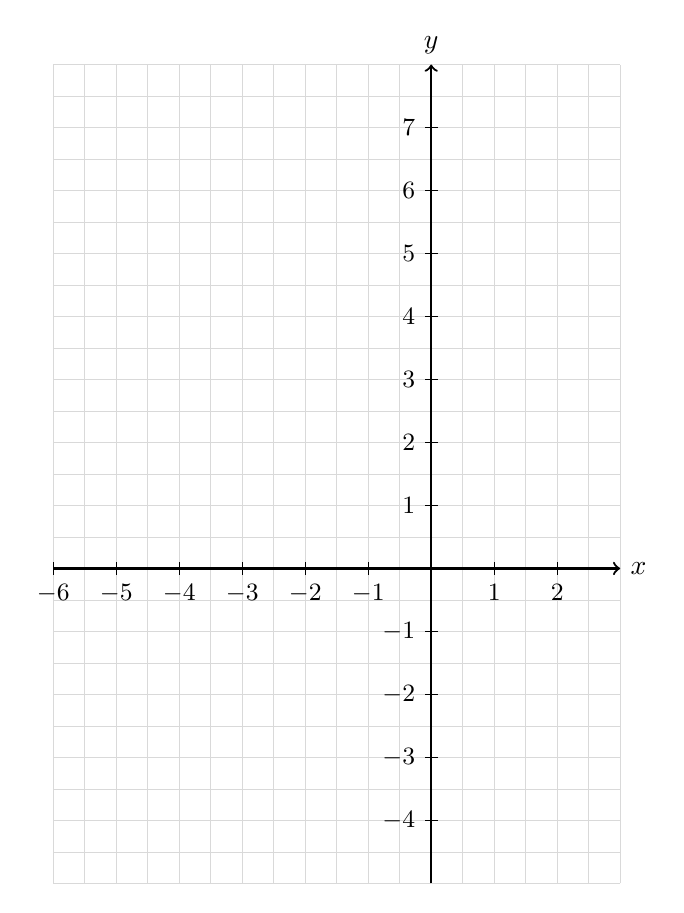
\begin{tikzpicture}[scale=0.8]
				% Grid
				\draw[step=0.5cm, gray!30, very thin] (-6,-5) grid (3,8);
				% Axes
				\draw[thick,->] (-6,0) -- (3,0) node[right] {$x$};
				\draw[thick,->] (0,-5) -- (0,8) node[above] {$y$};
				% Axis labels
				\foreach \x in {-6,-5,-4,-3,-2,-1,1,2}
					\draw (\x,0.1) -- (\x,-0.1) node[below] {\small $\x$};
				\foreach \y in {-4,-3,-2,-1,1,2,3,4,5,6,7}
					\draw (0.1,\y) -- (-0.1,\y) node[left] {\small $\y$};
			\end{tikzpicture}
			\end{center}

			\newpage

			\textbf{Problem 9:}
            
            Graph $y = -x^2 + 4x - 3$ using your work from Problem 2.

			\vspace{0.5cm}

			\begin{center}
			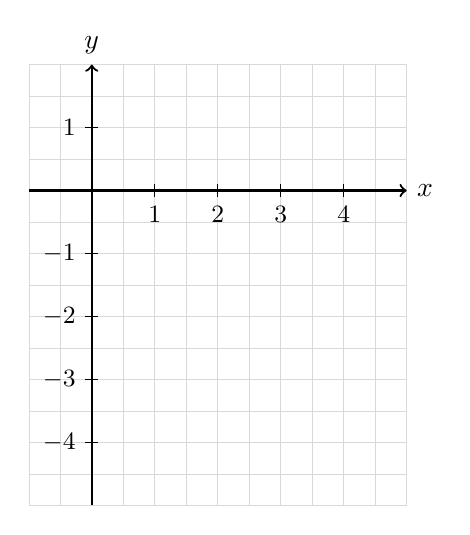
\begin{tikzpicture}[scale=0.8]
				% Grid
				\draw[step=0.5cm, gray!30, very thin] (-1,-5) grid (5,2);
				% Axes
				\draw[thick,->] (-1,0) -- (5,0) node[right] {$x$};
				\draw[thick,->] (0,-5) -- (0,2) node[above] {$y$};
				% Axis labels
				\foreach \x in {1,2,3,4}
					\draw (\x,0.1) -- (\x,-0.1) node[below] {\small $\x$};
				\foreach \y in {-4,-3,-2,-1,1}
					\draw (0.1,\y) -- (-0.1,\y) node[left] {\small $\y$};
			\end{tikzpicture}
			\end{center}

			\newpage

		\subsection*{Part D: Complete Analysis}

			For the following functions, find all key features AND sketch the graph.\\\\

			\textbf{Problem 10:}
            
            $y = x^2 - 4x$

			\vspace{0.5cm}

			Direction: \underline{\hspace{2in}}

			$y$-intercept: \underline{\hspace{2in}}

			Axis of symmetry: \underline{\hspace{2in}}

			Vertex: \underline{\hspace{2in}}

			$x$-intercepts: \underline{\hspace{2in}}

			\vspace{0.5cm}

			\begin{center}
			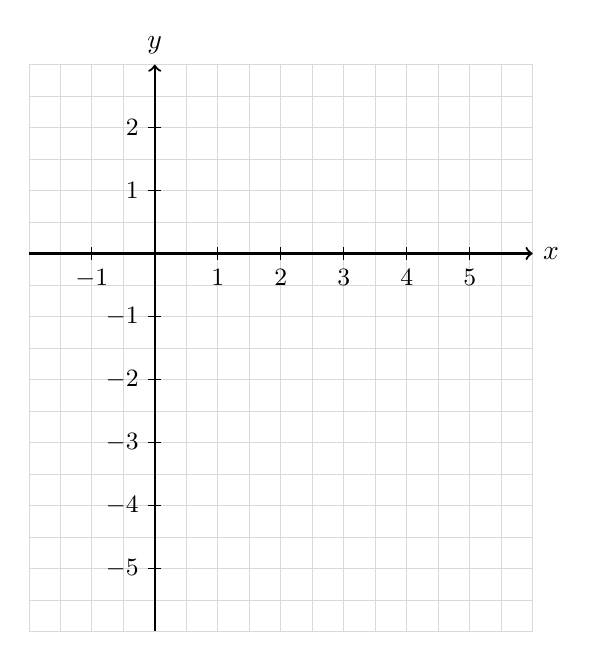
\begin{tikzpicture}[scale=0.8]
				% Grid
				\draw[step=0.5cm, gray!30, very thin] (-2,-6) grid (6,3);
				% Axes
				\draw[thick,->] (-2,0) -- (6,0) node[right] {$x$};
				\draw[thick,->] (0,-6) -- (0,3) node[above] {$y$};
				% Axis labels
				\foreach \x in {-1,1,2,3,4,5}
					\draw (\x,0.1) -- (\x,-0.1) node[below] {\small $\x$};
				\foreach \y in {-5,-4,-3,-2,-1,1,2}
					\draw (0.1,\y) -- (-0.1,\y) node[left] {\small $\y$};
			\end{tikzpicture}
			\end{center}

			\newpage

		\subsection*{Part E: Word Problems}

			\textbf{Problem 11:}

			A toy rocket is launched from the ground.

			Its height $h$ in feet after $t$ seconds is given by:

			$h = -16t^2 + 64t$\\

			\textbf{Part A:}
            
            Find the axis of symmetry.

			\vspace{1cm}

			\textbf{Part B:}
            
            Find the vertex. What does the vertex represent in this context?

			\vspace{1cm}

			\textbf{Part C:}
            
            Find the $t$-intercepts. What do they represent in this context?

			\vspace{1cm}

			\textbf{Part D:}
            
            Sketch the graph of the rocket's height.

			\begin{center}
			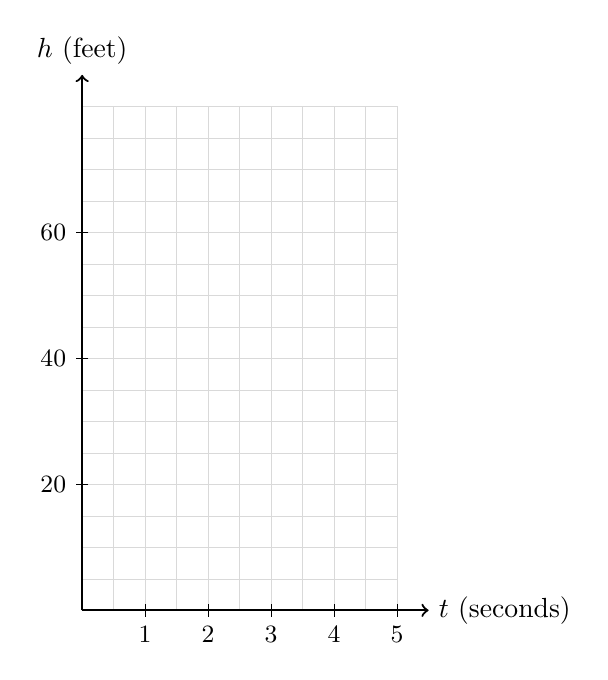
\begin{tikzpicture}[scale=0.8]
				% Grid
				\draw[step=0.5cm, gray!30, very thin] (0,0) grid (5,8);
				% Axes
				\draw[thick,->] (0,0) -- (5.5,0) node[right] {$t$ (seconds)};
				\draw[thick,->] (0,0) -- (0,8.5) node[above] {$h$ (feet)};
				% Axis labels
				\foreach \x in {1,2,3,4,5}
					\draw (\x,0.1) -- (\x,-0.1) node[below] {\small $\x$};
				\foreach \y in {20,40,60}
					\draw (0.1,\y/10) -- (-0.1,\y/10) node[left] {\small $\y$};
			\end{tikzpicture}
			\end{center}

			\newpage

			\textbf{Problem 12:}

			A ball is thrown from a height of 6 feet.

			Its height $h$ in feet after $t$ seconds is given by:

			$h = -16t^2 + 32t + 6$\\

			\textbf{Part A:}
            
            Find the maximum height of the ball and when it occurs.

			\vspace{2cm}

			\textbf{Part B:}
            
            What is the initial height of the ball (when $t = 0$)?

			\vspace{2cm}

			\textbf{Part C:}
            
            Sketch the graph showing the ball's path.

			\begin{center}
			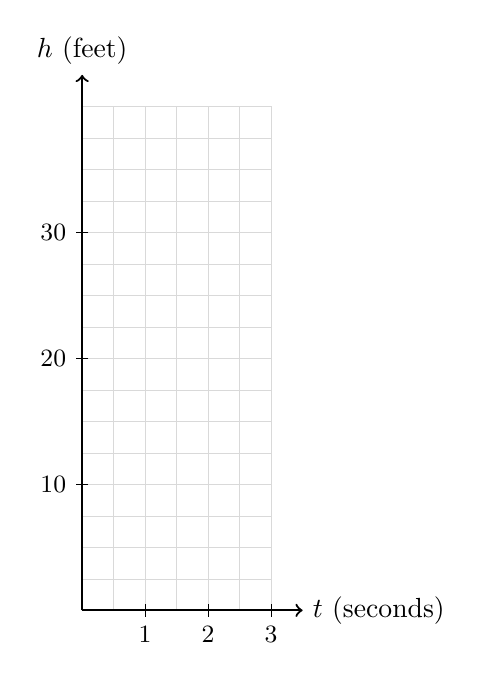
\begin{tikzpicture}[scale=0.8]
				% Grid
				\draw[step=0.5cm, gray!30, very thin] (0,0) grid (3,8);
				% Axes
				\draw[thick,->] (0,0) -- (3.5,0) node[right] {$t$ (seconds)};
				\draw[thick,->] (0,0) -- (0,8.5) node[above] {$h$ (feet)};
				% Axis labels
				\foreach \x in {1,2,3}
					\draw (\x,0.1) -- (\x,-0.1) node[below] {\small $\x$};
				\foreach \y in {10,20,30}
					\draw (0.1,\y/5) -- (-0.1,\y/5) node[left] {\small $\y$};
			\end{tikzpicture}
			\end{center}

            \newpage

	\section*{Session 10.2: \\ Solve by Square Roots; Completing the Square Setup}

	\section*{Quick Reference: Solving by Square Roots}

		\subsection*{Square Root Property}

			If $x^2 = k$, then $x = \pm\sqrt{k}$

			Remember: When you take the square root, you get both positive and negative solutions!

		\subsection*{Solving $(x - h)^2 = k$}

			\textbf{Steps:}
			\begin{enumerate}
				\item Take the square root of both sides: $x - h = \pm\sqrt{k}$
				\item Solve for $x$: $x = h \pm\sqrt{k}$
				\item Write two solutions: $x = h + \sqrt{k}$ or $x = h - \sqrt{k}$
			\end{enumerate}

		\subsection*{Introduction to Completing the Square}

			Goal: Rewrite $x^2 + bx$ as a perfect square trinomial

			\textbf{Perfect Square Trinomial Pattern:}

			$x^2 + bx + \left(\frac{b}{2}\right)^2 = \left(x + \frac{b}{2}\right)^2$

			\textbf{Key Idea:} Take half of the $x$-coefficient, then square it.

			To complete the square for $x^2 + bx$:
			\begin{enumerate}
				\item Find $\frac{b}{2}$
				\item Square it: $\left(\frac{b}{2}\right)^2$
				\item Add this value to create: $x^2 + bx + \left(\frac{b}{2}\right)^2$
				\item Factor as: $\left(x + \frac{b}{2}\right)^2$
			\end{enumerate}

		\newpage

	\section*{Homework 10.2: \\ Solve by Square Roots; Completing the Square Setup}

		\subsection*{Part A: Solve Using Square Roots}

			Solve each equation. Give exact answers (leave in square root form).\\\\

			\textbf{Problem 1:}
            
            $x^2 = 25$

			\vspace{3cm}

			\textbf{Problem 2:}
            
            $x^2 = 18$

			\vspace{3cm}

			\textbf{Problem 3:}
            
            $x^2 - 49 = 0$

			\vspace{3cm}

			\textbf{Problem 4:}
            
            $3x^2 = 75$

			\newpage

		\subsection*{Part B: Solve $(x - h)^2 = k$}

			Solve each equation. Give exact answers.\\\\

			\textbf{Problem 5:}
            
            $(x - 3)^2 = 16$

			\vspace{4cm}

			\textbf{Problem 6:}
            
            $(x + 5)^2 = 9$

			\vspace{4cm}

			\textbf{Problem 7:}
            
            $(x - 2)^2 = 7$

			\newpage

			\textbf{Problem 8:}
            
            $(x + 1)^2 - 20 = 0$

			\vspace{4cm}

		\subsection*{Part C: Complete the Square (Setup Only)}

			For each expression, find the value needed to complete the square.\\

			Then write the perfect square trinomial and its factored form.\\\\

			\textbf{Problem 9:}
            
            $x^2 + 8x + $ \underline{\hspace{1in}}

			\vspace{1cm}

			Value to add: \underline{\hspace{2in}}

			Perfect square trinomial: \underline{\hspace{2in}}

			Factored form: \underline{\hspace{2in}}

			\vspace{2cm}

			\textbf{Problem 10:}
            
            $x^2 - 10x + $ \underline{\hspace{1in}}

			\vspace{1cm}

			Value to add: \underline{\hspace{2in}}

			Perfect square trinomial: \underline{\hspace{2in}}

			Factored form: \underline{\hspace{2in}}

			\newpage

			\textbf{Problem 11:}
            
            $x^2 + 6x + $ \underline{\hspace{1in}}

			\vspace{1cm}

			Value to add: \underline{\hspace{2in}}

			Perfect square trinomial: \underline{\hspace{2in}}

			Factored form: \underline{\hspace{2in}}

			\vspace{2cm}

			\textbf{Problem 12:}
            
            $x^2 - 14x + $ \underline{\hspace{1in}}

			\vspace{1cm}

			Value to add: \underline{\hspace{2in}}

			Perfect square trinomial: \underline{\hspace{2in}}

			Factored form: \underline{\hspace{2in}}

			\newpage

		\subsection*{Part D: Word Problem}

			\textbf{Problem 13:}\\

			A square picture frame has an area of 80 square inches.\\

			\textbf{Part A:}
            
            Write an equation for the side length $s$ in inches.

			\vspace{2cm}

			\textbf{Part B:}
            
            Solve for $s$ using square roots. Give both the exact and approximate answer (round to one decimal place).

			\vspace{4cm}

			\textbf{Part C:}
            
            Which solution makes sense in this context?

			\newpage

	\section*{Session 10.3: \\ Completing the Square to Solve; Vertex Form}

	\section*{Quick Reference: Completing the Square to Solve}

		\subsection*{Steps to Solve $ax^2 + bx + c = 0$ by Completing the Square}

			\textbf{Step 1:} Move constant to the right side

			$ax^2 + bx = -c$

			\textbf{Step 2:} If $a \neq 1$, divide everything by $a$

			$x^2 + \frac{b}{a}x = -\frac{c}{a}$

			\textbf{Step 3:} Complete the square on the left side
			\begin{itemize}
				\item Take half of the $x$-coefficient: $\frac{1}{2} \cdot \frac{b}{a} = \frac{b}{2a}$
				\item Square it: $\left(\frac{b}{2a}\right)^2$
				\item Add to both sides
			\end{itemize}

			\textbf{Step 4:} Factor the left side as a perfect square

			\textbf{Step 5:} Solve using square roots

		\subsection*{Converting to Vertex Form}

			Standard form: $y = ax^2 + bx + c$

			Vertex form: $y = a(x - h)^2 + k$ where $(h, k)$ is the vertex

			\textbf{Process:}
			\begin{enumerate}
				\item If $a \neq 1$, factor out $a$ from the $x$-terms only
				\item Complete the square inside the parentheses
				\item Simplify to get vertex form
			\end{enumerate}

			\textbf{Reading the vertex:} In $y = a(x - h)^2 + k$, the vertex is $(h, k)$

			Note the sign! $y = (x - 3)^2 + 5$ has vertex $(3, 5)$, not $(-3, 5)$

		\newpage

	\section*{Homework 10.3: \\ Completing the Square to Solve; Vertex Form}

		\subsection*{Part A: Solve by Completing the Square}

			Solve each equation by completing the square. Show all steps.\\\\

			\textbf{Problem 1:}
            
            $x^2 + 6x + 5 = 0$

			\vspace{5cm}

			\textbf{Problem 2:}
            
            $x^2 - 8x + 12 = 0$

			\newpage

			\textbf{Problem 3:}
            
            $x^2 + 4x - 5 = 0$

			\vspace{5cm}

			\textbf{Problem 4:}
            
            $x^2 + 10x = -9$

			\newpage

		\subsection*{Part B: Solve When $a \neq 1$}

			Solve by completing the square. Remember to divide by $a$ first!\\\\

			\textbf{Problem 5:}
            
            $2x^2 + 8x - 10 = 0$

			\vspace{6cm}

			\textbf{Problem 6:}
            
            $3x^2 - 12x + 9 = 0$

			\newpage

		\subsection*{Part C: Convert to Vertex Form}

			Rewrite each function in vertex form by completing the square.\\

			Then identify the vertex.\\\\

			\textbf{Problem 7:}
            
            $y = x^2 + 8x + 10$

			\vspace{5cm}

			Vertex form: \underline{\hspace{3in}}

			Vertex: \underline{\hspace{2in}}

			\newpage

			\textbf{Problem 8:}
            
            $y = x^2 - 6x + 5$

			\vspace{5cm}

			Vertex form: \underline{\hspace{3in}}

			Vertex: \underline{\hspace{2in}}

			\vspace{2cm}

			\textbf{Problem 9:}
            
            $y = x^2 + 4x - 1$

			\vspace{5cm}

			Vertex form: \underline{\hspace{3in}}

			Vertex: \underline{\hspace{2in}}

			\newpage

		\subsection*{Part D: Convert When $a \neq 1$}

			Rewrite in vertex form. Factor out $a$ from the $x$-terms first!\\\\

			\textbf{Problem 10:}
            
            $y = 2x^2 + 8x + 3$

			\vspace{6cm}

			Vertex form: \underline{\hspace{3in}}

			Vertex: \underline{\hspace{2in}}

			\newpage

			\textbf{Problem 11:}
            
            $y = -x^2 + 6x - 5$

			\vspace{6cm}

			Vertex form: \underline{\hspace{3in}}

			Vertex: \underline{\hspace{2in}}

			\newpage

		\subsection*{Part E: Word Problem}

			\textbf{Problem 12:}\\

			A ball is thrown upward from a height of 4 feet.\\

			Its height $h$ in feet after $t$ seconds is given by:\\

			$h = -16t^2 + 32t + 4$

			\vspace{0.5cm}

			\textbf{Part A:}
            
            Rewrite the equation in vertex form by completing the square.

			\vspace{6cm}

			\textbf{Part B:}
            
            What is the maximum height of the ball? At what time does it reach this height?

			\vspace{3cm}

			\textbf{Part C:}
            
            Explain what the vertex represents in this context.

			\newpage

	\section*{Unit 10 Quiz: Quadratic Graphs \& Completing the Square}

		\subsection*{Section 1: Key Features of Quadratics}

			For the function $y = x^2 - 4x + 3$, find:

			\vspace{0.5cm}

			\textbf{Problem 1:}
            
            Direction (opens up or down)

			\vspace{2cm}

			\textbf{Problem 2:}
            
            $y$-intercept

			\vspace{2cm}

			\textbf{Problem 3:}
            
            Axis of symmetry

			\vspace{3cm}

			\textbf{Problem 4:}
            
            Vertex (show your work)

			\newpage

		\subsection*{Section 2: Solve by Square Roots}

			Solve each equation. Give exact answers.\\\\

			\textbf{Problem 5:}
            
            $x^2 = 36$

			\vspace{3cm}

			\textbf{Problem 6:}
            
            $(x - 4)^2 = 25$

			\vspace{4cm}

			\textbf{Problem 7:}
            
            $(x + 2)^2 = 12$

			\newpage

		\subsection*{Section 3: Complete the Square}

			\textbf{Problem 8:}\\

			What value completes the square for $x^2 + 10x + $ \underline{\hspace{1in}} ?

			\vspace{2cm}

			Write the perfect square trinomial and factor it.

			\vspace{3cm}

		\subsection*{Section 4: Solve by Completing the Square}

			\textbf{Problem 9:}\\

			Solve $x^2 + 8x + 7 = 0$ by completing the square. Show all steps.

			\newpage

		\subsection*{Section 5: Vertex Form}

			\textbf{Problem 10:}\\

			Rewrite $y = x^2 + 6x + 4$ in vertex form.

			\vspace{6cm}

			\textbf{Problem 11:}\\

			What is the vertex of $y = (x - 5)^2 + 3$?

			\vspace{2cm}

		\subsection*{Section 6: Word Problem}

			\textbf{Problem 12:}\\

			A diver jumps from a platform.\\

			Her height $h$ in feet above the water after $t$ seconds is:\\

			$h = -16t^2 + 8t + 24$

			\vspace{0.5cm}

			Find the maximum height of the diver and the time when she reaches it.

			\newpage

\end{document}